\chapter{\IfLanguageName{dutch}{Stand van zaken}{State of the art}}%
\label{ch:stand-van-zaken}

% Tip: Begin elk hoofdstuk met een paragraaf inleiding die beschrijft hoe
% dit hoofdstuk past binnen het geheel van de bachelorproef. Geef in het
% bijzonder aan wat de link is met het vorige en volgende hoofdstuk.

% Pas na deze inleidende paragraaf komt de eerste sectiehoofding.

\section{\IfLanguageName{dutch}{Enterprise Resource Planning}{Enterprise Resource Planning}}%
\label{sec:erp}
Enterprise Resource Planning (ERP) is een systeem dat is ontwikkeld om alle divisies in een bedrijf te integreren, zodat het een effectief en efficiënt bedrijfsproces wordt \autocite{Wardhanaa2022}. Een organisatie heeft vier functionele gebieden, namelijk Marketing en Verkoop, Supply Chain Managament (CSM), Accounting en Financiën en Human Resources (HR).
Het is een computer gebaseerd hulpmiddel dat verschillende bedrijfsprocessen kan verenigen en de informatie kan structureren in een geavanceerde datastructuur-entiteit \autocite{Xulu2020}. Een ERP-systeem wordt gezien als een methode om de opslag en het gebruik van relevante bedrijfsgegevens te systematiseren door middel van geautomatiseerde elementen. Er wordt verwacht dat ERP-systemen worden toegepast als planningssystemen. Als gevolg hiervan kunnen ERP-systemen weliswaar effectieve  planningshulpmiddelen zijn, maar ze kunnen ook voor andere doeleinden gebruikt worden, waaronder de analyse van gegevens die de dagelijkse besluitvorming kunnen vergemakkelijken om negatieve bedrijfsresultaten te voorkomen of te profiteren van dagelijkse kansen die zich dynamisch kunnen voordoen.
Om ERP effectief te laten werken, is het absoluut noodzakelijk dat de werknemers, die ERP-gebruikers zijn, tevreden zijn met het systeem om het effectief te kunnen gebruiken.

\subsection{Odoo}
Odoo is een eenvoudig te gebruiken alles-in-één beheersoftware van ERP. Odoo biedt verschillende geïntegreerde applicatiemodules, zoals de inventarismodule, de boekhoudmodule, e-commerce, marketing, enzovoort \autocite{Wardhanaa2022}. Het voordeel van het gebruik van een Odoo-software is dat deze eenvoudig gebruikt kan worden en dat alle divisies in het bedrijf geïntegreerd zijn. Odoo ERP-software maakt voornamelijk gebruik van de programmeertalen Phyton, XML en JavaScript.

\subsection{SAP}
SAP is de topleider in de wereld van het leveren van ERP service \autocite{WatSAP}. Het is een softwareprogramma dat door veel bedrijven gebruikt wordt \autocite{Indeed2023}. De geïntegreerde applicaties verbinden alle bedrijfsonderdelen met een intelligente suite op een volledig digitaal platform. Ook wordt het toegepast om informatie-uitwisseling en dataverwerking tussen verschillende organisaties te faciliteren. Daarbij wordt het oude, proces gestuurde platform vervangen. SAP ontwikkelt softwareoplossingen die worden gebruikt door kleine bedrijven, middelgrote bedrijven en grote bedrijven.
SAP is een soort software dat veel bedrijven gebruiken om de dagelijkse activiteiten en processen, zoals boekhouding en projectbeheer, te besturen. In het kort geeft SAP bedrijven de mogelijkheid om al deze processen te centraliseren zodat elke afdeling toegang heeft tot de benodigde gegevens en bestanden. Dit zorgt er onder meer voor dat werknemers hun werk efficiënter kunnen uitvoeren.

\section{\IfLanguageName{dutch}{Master Data}{Master Data}}%
\label{sec:masterdata}
Master data omvat de belangrijkste gegevens klanten, producten, diensten, personeel, technologie, materialen, enzovoort \autocite{Prokhorov2018}. Deze gegevens zijn het cruciaalst om de bedrijfsprocessen van een bedrijf optimaal te laten verlopen. Andere namen voor master data zijn brondata of stamdata. Master data bevindt zich in verschillende applicaties van het ERP-systeem, namelijk Customer Relationship Management (CRM), logistiek, productie of administratie. Master gegevens worden relatief zelden gewijzigd en zijn niet transactioneel.
Masterdata vormen doorgaans slechts een klein percentage van alle bedrijfsgegevens, maar het behoort tot de meest complexe en waardevolste gegevens van een organisatie \autocite{SAPMasterData}. 
Enkele voorbeelden van stamgegevens zijn: 

\begin{figure}[htbp]
  \centering
  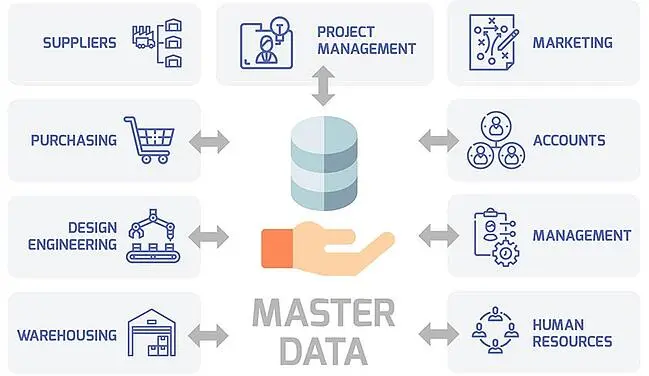
\includegraphics[scale=0.5]{../images/Master-Data.png}
  \caption{Master Data}
\end{figure}

\subsection{Customer master data}
Het bevat de stamgegevens van de klanten, alle kerngegevens die nodig zijn om zaken te doen met de klanten. Van de contactgegevens tot de aankoopgeschiedenis en de betalingsvoorwaarden. Het beheren van de master data voor dit domein omvat het opschonen en standaardiseren van de gegevens in Enterprise Resource Planning-, Customer Relationship Management- en andere systemen.

\subsection{Supplier master data}
Master gegevens van leveranciers omvatten gegevens voor leveranciersaccounts, contracten, beleid, prijzen en meer. Het vormt het middelpunt van alle belangrijke inkoopactiviteiten, van planning, het verkrijgen van een offerte en inkoop. Opgeschoonde en vertrouwde masterdata van leveranciers zijn van cruciaal belang voor het beantwoorden van vragen over bijvoorbeeld leveranciersuitgaven, prijzen en presentaties. 

\subsection{Location master data}
Locatie master data heeft belangrijke kenmerken met betrekking tot de fysieke locaties van agentschappen, bedrijfskantore, distributiecentra en winkels. Deze gegevens zijn allemaal opgenomen in de locatiegegevens van een organisatie. Eenmaal verbonden met andere datadomeinen kan deze informatie helpen bij het nemen van locatie gebaseerde beslissingen, zoals het bepalen van het juiste productassortiment voor een bepaalde winkel.

\subsection{Product master data}
Het beheer van product master data omvat attributen zoals productnummer, categorie, prijs, details en alle andere noodzakelijk gegevens. Omdat deze gegevens in verschillende processen voor verkoop, marketing, toeleveringsketen en de levenscyclus van productontwikkeling kunnen gebruikt worden, moeten deze gegevens zeer betrouwbaar en nauwkeurig zijn.

\subsection{Asset master data}
Stamgegevens van assets beschrijven de vaste en immateriële activa in een bedrijf, zoals inventaris, apparatuur en handelsmerken. Het bevat meestal attributen zoals afschrijvingsvoorwaarden en activaklassen, lease-informatie en meer. Onnauwkeurige masterdata van assets kunnen leiden tot ondermaats gebruik en beheer van deze assets.

\section{\IfLanguageName{dutch}{Master Data Managament}{Master Data Management}}%
\label{sec:mdm}
Master Data Management (MDM) richt zich voornamelijk op het beheer van de master data \autocite{Martins2022}. Om de communicatie tussen de verschillende applicaties mogelijk te maken, is het noodzakelijk dat de master data eenduidig wordt opgeslagen en met elkaar in verband wordt gebracht. 

Het doel van MDM is om ervoor te zorgen dat er geen repetitieve, onvolledige en inconsistente gegevens zijn op verschillende gebieden van de activiteiten van de organisatie \autocite{Prokhorov2018}. De basisbenadering van MDM omvat processen als het verzamelen, accumuleren, opschonen van gegevens, vergelijken ervan, consolideren, kwaliteitscontrole en gegevensdistributie in de organisatie. Hierdoor worden de daaropvolgende consistentie en controle van het gebruik in verschillende operationele en analytische toepassingen gewaarborgd.

MDM is praktisch onmisbaar in grote ondernemingen en in bedrijven die blijven groeien. Als bedrijven blijven groeien nemen het aantal applicaties, gegevens en hun eindgebruikers toe. Omdat MDM-oplossingen steeds toegankelijker worden voor kleinere organisaties, profiteren ook zij in toenemende mate van de voordelen van Master Data Management.

\begin{figure}[htbp]
  \centering
  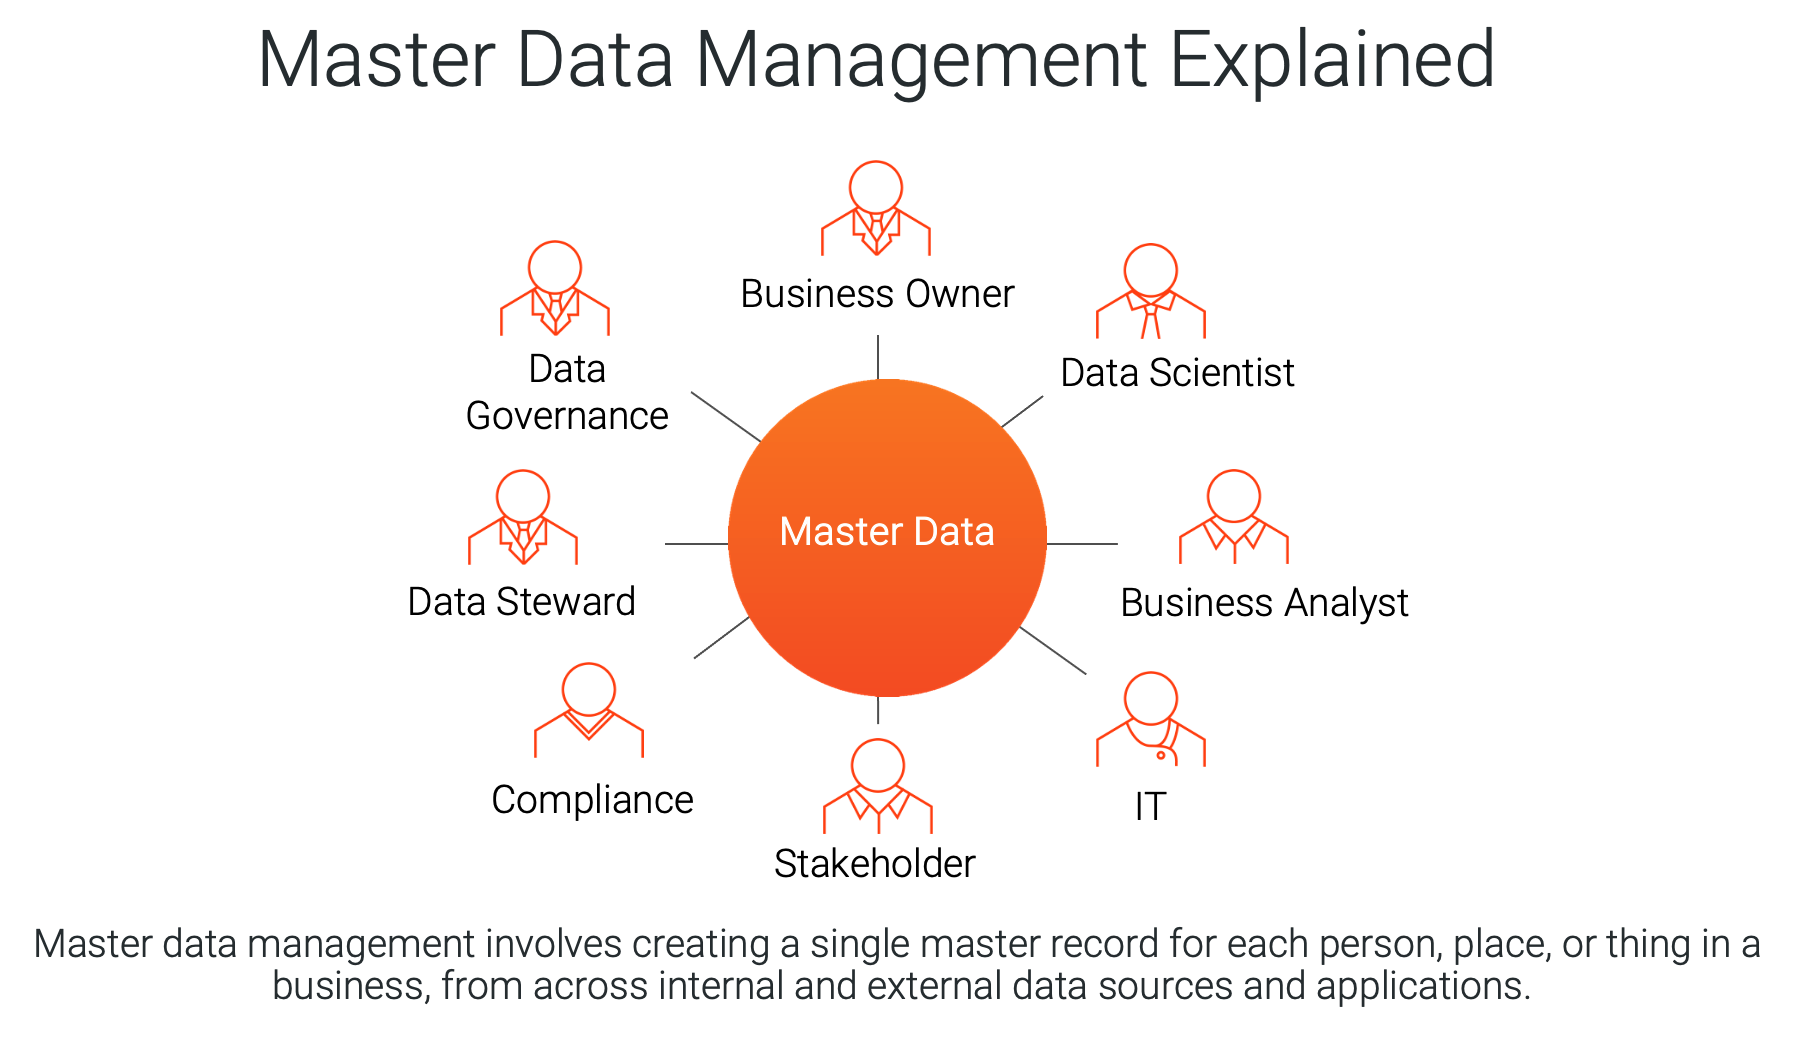
\includegraphics[scale=0.2]{../images/MasterData.png}
  \caption{Master Data Managament}
\end{figure}

\subsection{Voordelen Master Data Management}
Volgens het onderzoek van \textcite{Pansara2024}, waarin hij de strategieën voor Master Data Management (MDM)-Integration bespreekt en ook de voordelen ervan, biedt MDM een baanbrekende strategie die verschillende voordelen biedt voor bedrijven die de waarde van hun data-assets willen maximaliseren.

\subsubsection{Betere datakwaliteit}
De integratie van MDM is een krachtig hulpmiddel om de datakwaliteit binnenin een onderneming naar voorheen ongehoorde hoogten te verbeteren. Organisaties creëren één enkele, gezaghebbende vorm voor master data door middel van consolidatie, federatie of adoptie van een co-extensiemodel. Dankzij deze gecentraliseerde methode worden uniformiteit, nauwkeurigheid en consistentie verzekerd voor alle master data-instanties. Door het oplossen van conflicten en het minimaliseren van dubbele records wordt er een betrouwbare en uitstekende databasis uitgebouwd. Wanneer ook besluitvormers vertrouwen op deze nauwkeurige en betrouwbare gegevens, versterkt dit een verbeterende gegevenskwaliteit in het bedrijf tegen fouten, het vergroot ook de geloofwaardigheid en wekt het vertrouwen in hen.

\subsubsection{Namen van kennisbeslissingen}
Het nemen van goed geïnformeerde, data gestuurde beslissingen is hoofdzakelijk afhankelijk van MDM-integratie. Bedrijven kunnen barrières verwijderen en de besluitvormers een alomvattend beeld weergeven van essentiële informatie die door masterdata te verkrijgen is. Leidinggevenden kunnen goed geïnformeerde strategische beslissingen nemen door grondig inzicht te verwerven in de omgeving van hun organisatie. Wanneer zij dan toegang hebben tot de betrouwbare en consistente gegevens kunnen beslissingen doordachter gemaakt worden. Door MDM werken besluitvormers allemaal op verschillende afdelingen met dezelfde, meeste recente informatie. Dit bevordert een masterdata-integratie cross-functionele samenwerking. Hierdoor wordt de integratie van MDM een essentieel onderdeel bij het coördineren van organisatiedoelen en het ontwikkelen van op een bewijs gebaseerde besluitvormingscultuur.

\subsubsection{Efficiënte bedrijfsvoering }

Nieuwe niveaus van efficiëntie worden bereikt door de ripple effects van MDM-integratie in het operationele landschap van een organisatie. Bij ripple effects wordt het databeheer gestroomlijnd, redundanties worden geëlimineerd en de tijd en moeite die nodig is voor data-onderhoud wordt verminderd dankzij het gecentraliseerde beheer van master data. De integratie van MDM verkleint de kans op fouten die worden veroorzaakt door onder andere inconsistentie of verouderde gegevens, hetzij door co-extensie, federatie of consolidatie. Verschillende bedrijfsactiviteiten maken deel uit van deze operationele stroomlijning, waardoor resource-efficiëntie en workflow optimalisatie worden gegarandeerd. Als uiteindelijk doel creëert MDM de omstandigheden waarin een bedrijf soepel kan functioneren, met meer flexibiliteit en reactievermogen op veranderende marktomstandigheden.

\subsubsection{Flexibiliteit en uitbreidbaarheid}
Bedrijven die Master Data Management integreren, zijn beter uitgerust om met veranderende bedrijfsomstandigheden om te gaan vanwege hun grotere schaalbaarheid en aanpassingsvermogen. Het vermogen om zonder moeite nieuwe databronnen te integreren, zich aan te passen aan veranderende bedrijfsvereisten en om te gaan met evoluerende dataformaten wordt steeds belangrijker naarmate bedrijven zich ontwikkelen en diversifiëren. De integratie van MDM biedt een fundament die flexibele genoeg is om mee te veranderen met de zakelijke ecosystemen, waardoor deze zowel aanpasbaar als schaalbaar is. MDM garandeert deze schaalbaarheid waarbij bedrijven met vertrouwen hun activiteiten kunnen laten groeien, de digitale transformaties kunnen omarmen en de allernieuwste technologie kunnen integreren.

\subsection{Best practices Master Data Management}
Een veel voorkomende misvatting volgens \textcite{Raghavendra2023} is dat het masterdata managementproces consistent en succesvol hoogwaardige master data zal opleveren. Echter, een slechte planningen uitvoering kunnen de kwaliteit van de bedrijfsgegevens verarmen. Daarom zijn datastandaardisatie, scrubbing en matchingstrategieën onmisbaar voor elke masterdata managementoplossing om een echte waarde te kunnen leveren.
Hier volgen enkele best practices van \textcite{Raghavendra2023} en \textcite{Sharma2023} voor master data beheer die kunnen helpen het beste uit MDM-integratie te halen:

\subsubsection{Plan goed}
Voldoende tijd investeren in het evalueren van de verschillende MDM-tools is van cruciaal belang. De businesscases moeten geplant en begrepen zijn voordat de perfecte oplossing voor de behoeften geselecteerd kan worden. Een goed in kaart gebrachte business case is cruciaal bij het kiezen en implementeren van een effectief instrument, ook moete het naadloos de bestaande technologieën integreren.

\subsubsection{Focus op de architectuur}
Integratie en synchronisatie zijn de twee meest essentiële aspecten van MDM. Het zorgt ervoor dat de integratiestrategie van de vooropgestelde oplossing werkt. Integratie van databronnen, zoals big data, is cruciaal voor de schaalbaarheid. MDM kan ook batch-integratie- en realtime-integratie-elementen samenvoegen. Elke integratiestrategie die de MDM hanteert, zal efficiënt zijn in het synchroniseren van de gegevens terug naar de bron.

\subsubsection{Juiste team op de juiste plek}
MDM is een zeer gespecialiseerde niche. Of het hele proces nu wordt uitbesteedt, een tool wordt aangeschaft of het allemaal in eigen beheer wordt gedaan: er moet voor gezorgd worden dat er een gekwalificeerd team aan boord is. De beste keuze is om een team samen te stellen met experts op het gebied van IT, belangrijke belanghebbenden in het bedrijf en de leveranciers. Dit zal een holistische benadering van MDM garanderen.

\subsubsection{Gefaseerde aanpak van de implementatie}
Wanneer men een overzicht maakt van wat er onmiddellijk allemaal gedaan moet worden en wat later gedaan moet worden, is dit een omvatrijke discipline. Door de juiste stappen in te stellen, is het mogelijk om met de juiste planning waardestijgingen te realiseren. Naarmate de bedrijfsprioriteiten veranderen, kan de implementatie worden herschikt om de meeste voordelen op te leveren.

\subsubsection{Voer frequente beoordelingen uit}
Het is essentieel om de resultaten van de MDM-strategie regelmatig te evalueren. De MDM-strategieën die waarde opleveren, kunnen worden opgeschaald of gewijzigd worden. Frequente beoordelingen kunnen kritische succesfactoren blijken te zijn.

\subsubsection{Verzamel maximale informatie}
Hoe meer gegevens er verzameld kunnen worden, hoe beter inzicht er verworven kan worden en hoe efficiëntere beslissingen er genomen kunnen worden om het succes van uw bedrijf te vergroten. Er moeten nieuwe manieren blijven ontdekt worden die kunnen helpen om de waardevollere gegevens van de klanten en concurrenten te verkrijgen, want met meer informatie kunnen er meer zakelijke kansen benut worden. Van zodra er duidelijkheid is over de hiaten in de organisatie zijn bestaande gegevensverzamelingsproces, kunnen de nieuwe strategieën geïmplementeerd worden om de waardevollere en betrouwbare gegevens te verzamelen.

\subsubsection{Overweeg masterdata voor meerdere domeinen}
Een goed mastertype wordt gebruikt om elk bedrijfsprobleem op te lossen. Er zijn verschillende typen masterdata of domeinen op één platform, waardoor er holische inzichten en zeer goede bedrijfsresultaten verzekerd worden. Vandaag de dag brengen verschillende bedrijven hun klanten en productmasterdata in silo’s. Ze laten hun supply chain, gebouwen, assets en werknemers data staan. Organisaties brengen de volledige gegevensbronnen zoals transactiegegevens of productgegevens in hun masterdatabeheer. Hierdoor kunnen ze de verborgen verbinddingen vinden van hun eigen bedrijf. Er kunnen meerdere functies met meerdere verbindingen tot stand gebracht worden als er een paar stamgegevenssilo’s gebruikt worden. Deze functies kunnen real-time bewerkingen op schaal mogelijk maken. Een uitstekend multidomein is ontworpen om master data van klanten, leveranciers, producten en werknemers op de locatie samen te brengen en het bedrijf het rendement te laten zien. 

\subsubsection{Databeheer is een integraal onderdeel}
De belangrijkste onderdelen van MDM zijn datakwaliteit en data governance. Om een uitstekend framework voor gegevensbeheer te hebben, moet het verschillende aspecten omvatten, zoals guardrails en een perfecte workflow voor cross-checking van de nauwkeurigheid en redundantie van de gegevens. Het koppelt met succes de nieuwe gegevens, die in het systeem binnenkomen, met de beste huidige records. Een geavanceerd MDM-platform automatiseert het grootste deel van dit werk met behulp van Artificiële Intelligentie en Machine Learning. Hierdoor kunnen gebruikers gebruik maken van de voordelen die gepaard gaan met masterdatabeheer, zonder extra werk dat nodig is om de kwaliteit ervan te garanderen. 
Data governance omvat de data stewards. Data stewards zijn van elementair belang bij het vaststellen van absolute regels om ervoor te zorgen data master data van hoge kwaliteit en accuraat is. 
Zakelijke gebruikers profiteren van deze gegevens. Het MDM-systeem moet eenvoudig en intuïtief zijn voor een zakelijke gebruiker, zodat het onmiddellijk kan worden gebruikt. De nieuwste Master Data Management-platforms worden gebruikt door zakelijke gebruikers of om de algehele matchingmodellen te trainen aan de hand van de data en de nauwkeurigheid van de datakwaliteit in de loop van de tijd te verbeteren.

\subsubsection{Datakwaliteit controleren}
Hoe meer data je bezit, hoe meer je de kwaliteit van deze data zal moeten controleren, want meer is niet altijd betrouwbaar. De ontvangen data moet worden gevalideerd door een reeks kwaliteitsborgingsprocessen te implementeren. Niet elk klein stukje data dat wordt ontvangen is waardevol. Hoewel de gebruiker de data zal invoert, versterkt hij ook de verkeerde gegevens. Om een betrouwbaarder beeld te krijgen in het MDM-systeem, is het dus van essentieel belang om de kwaliteit van de verzamelde gegevens voldoen te controleren. 

\subsubsection{Bouw MDM die voldoet aan de bedrijfsdoelstellingen}
Niet alleen de IT-afdeling is betrokken bij het implementeren van de algemene structuur en referentiegegevens van MDM. Als eigenaar van een bedrijf moet u goed op de hoogte zijn van alle bedrijfsdoelstellingen, hoe u verstandig met de kritische bedrijfsgegevens omgaat en hoe u uw bedrijfsdoelstellingen aan het MDM-team communiceert. Dit kan gedaan worden door de Key Performance Indicators (KPIs), de kwartaaldoelen, de financiële plannen, de vijfjarenplannen en andere zaken op één lijn te brengen binnen het bedrijf. MDM verbeterd de klantenervaringen, de conversiepercentages en verhoogt de omzet. Het helpt de klanten te segmenteren en hen snel te identificeren voor verschillende kanalen heen, de oplossingstijden van problemen verkort, de efficiëntie van processen verbetert, de rapportage voor naleving versnelt en de fraude of weglekken van de inkomsten.

\subsubsection{Bouw een schaalbare en gebruiksvriendelijke MDM-oplossing}
Uit MDM-praktijken is te blijken dat zakenmensen klein beginnen en hun gegevens duidelijk organiseren om vroegtijdige winst te behalen. Deze methode kan echter ook complicaties opleveren op mislukken als het masterdatabeheer niet op schaal is gebouwd.
Traditionele master data managementsystemen zijn opgebouwd als een monoliet en omvatten probleemopschaling. Een monoliet bestaat uit verschillende onderdelen maar vormt constructief één geheel. Geavanceerde master data managementsystemen zijn gebouwd op een schaalbare architectuur om een gefaseerde methode te ondersteunen of om de flexibiliteit te laten reageren op veranderende marktomstandigheden. 
Doordat de gebruikers van het MDM-systeem weten en onthouden dat het datamodel in de loop van de tijd verandering met zich meebrengt, wijzigen en slaan ze nieuwe elementen op volgens de vereisten van het flexibele datamodel.

\subsubsection{Implementeer een gemeenschappelijke metadatalaag}
Door de ontwikkeling en integratie van een gemeenschappelijke metadatalaag kan de informatie gedeeld worden via analytische en beheerplatforms. Hiermee kan de efficiëntie verhoogd worden in elk aspect van de applicatie- en gegevensverzameling. Het helpt ook bij het leren kennen van de markttrends voordat er gloednieuwe producten gelanceerd worden en te begrijpen hoe goed een sociale mediacampagne presteert. De metadatalaag stroomlijnt de meeste van de gegevensverzamelingsprocessen en biedt betekenisvolle gegevens die gemakkelijk te begrijpen en te gebruiken zijn.

\subsubsection{Zet één basis voor gegevensbeheer op voor uw masterdata}
Een andere best practices is het creëren van één basis voor gegevensbeheer voor de stamgegevens. Veel zakelijke gebruikers hebben toegang tot één weergave van de stamgegevens. Ze krijgen consistente en real-time informatie en inzichten. Het kan mogelijks zijn dat de gegevens die ingevoerd worden niet in real-time worden bijgewerkt, ookal worden de gegevens ingevoerd in een geïsoleerd MDM-systeem. Dit probleem kan overwonnen worden door de nieuwste masterdatabeheerpraktijken te volgen en de gewenste voordelen te behalen. Er is binnen een onderneming één datamanagementfundament nodig om wendbaar te zijn, maar ook om een snelle time-to-value te kunnen realiseren.
Hierbij kan graph technology aan de pas komen. Het legt de volledige relaties vast en zorgt dat er snelle zoekacties verricht kunnen worden. Elke organisatie richt zich op de transformatie van de klantervaring, de vaardigheid om de relaties te benutten en verbindingen in gegevens om operationele beslissen te nemen, hierbij kan graph technology van groot belang worden. 

\subsubsection{Organiseer de gegevens op een zinvolle manier}
Uit een ongestructureerd gegevensbeheer kan er geen of moeilijk inzicht verworven worden. Daarom is het dus van essentieel belang om de bedrijfsinformatie op een gestructureerde manier te ordenen en dat de gebruikers naadloos toegang hebben tot de benodigde gegevens om hun doelstellingen te bereiken. Door de gegevensopslag- en ophaalproces te vereenvoudigen kan er veel makkelijker de nodige zaken terug gevonden worden. Ook helpt het voornamelijk bij data-analisten, zij analyseren voortdurend de gegevens en kunnen niet veel tijd investeren in het zoeken naar de juiste gegevens. 

\subsubsection{Master gegevens moeten toegankelijk zijn voor verschillende teams}
In de bedrijfswereld worden voortdurend gegevens geproduceerd en geconsumeerd, daardoor maken verschillende zakelijke gebruikers gebruik van dezelfde gegevens. Het koppelen van verschillende soorten master data is essentieel om maximale inzichten te verkrijgen en iedereen data verantwoordelijk te maken. 

\subsubsection{Bied snelle toegang tot gegevens aan de juiste gebruiker}
Bij het hebben van goed georganiseerde gegevens kan er een eenvoudigere toegang veroorzaakt worden. Om het proces voor het ophalen van gegevens te verbeteren, moeten alle barrières tussen het personeel en de gegevens die zij nodig hebben weggenomen worden. Het vermijden van het instellen van complexe toegangsrechten kan hierbij als best practice opgenomen worden. Zo kunnen ze hun toegewezen taken uitvoeren. 

\subsubsection{Verbeter de beveiligingsnormen om cyberaanvallen aan te pakken}
Bedrijfsgegevens zijn het belangrijkste bezit van een organisatie, dus is het noodzakelijk dat deze gegevens veilig bewaard en beheerd worden. Er bestaan kansen dat er cyberaanvallen gebeuren en dat hackers alle gegevens wissen of dat deze gegevens in de handen terechtkomen van de concurrenten. In zo’n situatie kan je uw innovatieve voorsprong verliezen. Strategieën en hulpmiddelen voor gegevensbeveiliging moeten overwogen en geïmplementeerd orden zodat de kritieke bedrijfsinformatie zo goed mogelijk beschermd blijft. 

\subsubsection{Gegevens bewust bijwerken voor beveiligings- en privacybeheer}
Het uitgangspunt voor de regelgeving van gegevens privacy is GDPR.
General Data Protection Regulation (GDPR) is het beheer en de beveiliging van de persoonlijke gegevens van Europese burgers \autocite{Vlaanderen}. Sinds mei 2018 moet elk bedrijf kunnen aantonen welke persoongegevens ze verzamelen en hoe ze deze data gebruiken en beveiligen. Alle ogranisaties, overheidsdiensten en instellingen die in Europa persoongegevens verwerken, gebruiken, registeren of bewaren, moeten aan deze richtlijn voldoen. Er staan een aantal principes centraal in verband met de gegevensbescherming, deze staan ook al in de huidige regelgeveing, maar ze worden verstrekt in de nieuwe GDPR-regelgeving.
Bij een ouder masterdatasysteem met langzame updates heeft het systeem veel meer moeite om snel op de voorkeuren van de gebruiker te reageren. Als er te lang gewacht worden om het systeem te updaten, kan er een downtime nodig zien die misschien uren tot dagen kan duren om de beveiliging van de software weer optimaal te zetten. Een geavanceerd Master Data Management omvat automatische beveiligingsupdates op de achtergrond en verbonden met de klantengegevens. Sommige bedrijven hebben losgekoppelde of onsamenhangende klantgegevens die verspreid zijn over het hele bedrijfssysteem, hierbij is deze praktijk onmogelijk. Het hebben van een modern Software as a Service (SaaS) MDM-platform waarmee organisaties hun databeleid regelmatig kunnen bijwerken, is de beste oplossing voor het handhaven van een perfect beveiligings- en privacybeleid voor een bedrijf. Software as a Service is een softwaredistributie model waarbij een cloudprovider applicaties host en deze via het internet beschikbaar stelt aan de eindgebruikers \autocite{Chai2022}.

\subsubsection{Geef toegangsrechten voor rollen en rechten}
Het geven van toegangsrechten ondersteunt ook de gegevensbeveiliging. Er zijn verschillende niveaus van leidinggevenden nodig om toegang te verwerven tot een specifieke of verschillende dataset. Om de juiste gebruiker van de juiste informatie te voorzien, kunnen er rollen en rechten toegevoegd worden aan specifieke personen. Dit biedt ook ene voordeel met zich mee, namelijk dat u uw bedrijfsgegevens zo meer kunt beschermen omdat niet iedereen toegang heeft tot alle data. Wel moet iedereen van de organisatie op de hoogte zijn van zijn rollen en rechten zodat zij ook weten tot welke informatie zij toegang hebben. 

\subsubsection{Blijf de nieuwste technologische trends volgen }
Door gebruik te maken van de nieuwste technologieën kunnen de mogelijkheden van de Master Data Management oplossing verbeteren. Het bekijken en volgende van de nieuwste MDM-trends en geavanceerde technologieën om de gegevensbeveiliging, gegevensopschoning, verwijdering van dubbele gegevens en gegevensorganisatieprocessen sneller en eenvoudiger te verbeteren.

\subsection{Challenges Master Data Management}
Alhoewel  MDM veel voordelen biedt, is de integratie van MDM niet vlekkeloos te verrichten. Slechte kwaliteit of inconsistente gegevens tussen verschillende systemen kunnen een groot obstakel vormen voor integratie-inspanningen \autocite{Pansara2024}. Duplicaten, inconsistente gegevensformaten en onnauwkeurige gegevens kunnen het moeilijker maken om één betrouwbare opslagplaats voor hoofdgegevens te creëren. De integratie van MDM kan worden belemmerd door organisatorisch verzet tegen nieuwe procedures en technologie voor gegevensbeheer. Medewerkers die gewend zijn aan de huidige workflows of die zich zorgen maken over onderbrekingen kunnen een bron van weerstand zijn. Bedrijven worstelen vaak met ingewikkelde datalandschappen die een verscheidenheid aan dataformaten, -typen en -bronnen omvatten \autocite{Sharma2020}. Het omgaan met oude systemen, verschillende bedrijfseenheden en verschillende data governance-praktijken draagt bij aan de complexiteit.


\section{\IfLanguageName{dutch}{Master Data Governance}{Master Data Governance}}%
\label{sec:mdg}
Data governance is een ondernemingsbrede discipline met een enorme reikwijdte \autocite{Cawsey2022}. Master Data Governance (MDG) is nodig om nauwkeurige identificatie en bedrijfsrelevante verrijking van de activa tot stand te brengen. Activa in een bedrijf kan beschouwd worden tot alle bezittingen van het bedrijf \autocite{Informer2023}. 
In realiteit kan een data governance programma geïmplementeerd worden zonde een MDM-project uit te voeren, maar MDM kan niet geïmplementeerd worden zonder een aanzienlijk stukje data governance te doen  \autocite{Collibra2023}. Alle bedrijfsprogramma vereisen goede data en alle data heeft governance nodig. 
MDM creëert een raamwerk van regels, beleid en procedures gericht op het waarborgen van de kwaliteit en consistentie van bedrijfsgegevens \autocite{Shewaramani2023}. Het omvat verschillende componenten, waaronder definities, workflows, beleid en de afbakening van verantwoordelijkheden en rollen voor datagebruikers. Het hoofdzakelijkste doel van  MDM-gegevensbeheer is het handhaven van de nauwkeurigheid, volledigheid en onderline verbondenheid van gegevens in de hele organisatie. 

\begin{figure}[htbp]
  \centering
  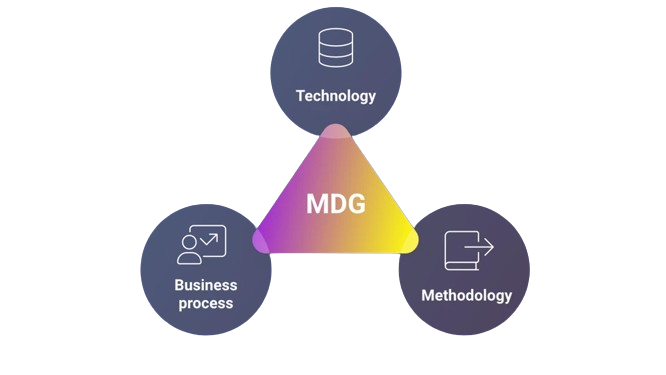
\includegraphics[scale=0.5]{../images/AlluvionMDG.png}
  \caption{Master Data Governance}
  \small\textbf{Copyright © 2024 Alluvion. All rights reserved.}
\end{figure}

\section{\IfLanguageName{dutch}{Artificial Intelligence}{Artificial Intelligence}}%
\label{sec:ai}
Kunstmatige Intelligentie (AI) en Machine Learning worden vaak door elkaar gebruikt, maar het zijn eigenlijk twee verschillende concepten die onder dezelfde paraplu vallen.

Volgens \textcite{Coursera2024} kan AI beschreven worden als een computersoftware die menselijke cognitieve vaardigheden nabootst om complexe taken uit te voeren. Deze taken konden vroeger alleen maar door de mensen uitgevoerd worden. Deze taken omvatten het verwerken van gegevens zoals een besluitvorming, een data-analyse en een taalvertaling. AI wordt omschreven als een code die computersystemen expliciet programmeert om taken uit te voeren waarvoor menselijk redeneren vereist is. Terwijl bij geautomatiseerde machines en systemen slechts een reeks instructies volgen en deze plichtsgetrouw en zonder verandering uitgevoerd worden. AI gedreven machines kunnen leren van deze interacties om hun prestaties en efficiëntie te verbeteren. 

\subsection{Machine Learning}
Machine learning is a subset of AI in which algorithms are trained on data sets to become machine learning models capable of performing specific tasks.  
Machine Learning (ML) is een deelgebied van kunstmatige intelligentie \autocite{Coursera2024}. ML richt zich op het trainen van machine learning-algoritmen met datasets om machine learning-modellen te produceren die complexe taken kunnen uitvoeren, zoals het sorteren van afbeeldingen, het voorspellen van verkopen of het analyseren van big data. Tegenwoordig is ML de belangrijkste manier waarop de meeste mensen omgaan met AI. ML worden vaak toegepast op volgende zaken: 

\begin{itemize}
  \item Het ontvangen van video-aanbevelingen op een online videostreamingplatform.
  \item	Online een probleem oplossen met een chatbot, die op basis van antwoorden naar de juist bronnen verwijst.
  \item	Het behulp van virtuele assistenten die reageren op verzoeken om vergaderingen in een agenda te plannen, een specifiek nummer laten afspreken of naar iemand bellen.
\end{itemize}

\subsection{Deep Learning}
Deep Learning (DL) is een subset van Machine Learning, waarbij kunstmatige neurale netwerken het menselijk brein nabootsen \autocite{Coursera2024a}. DL wordt gebruikt om complexere redeneringstaken uit te voeren zonder een menselijke tussenkomst. Het bestaat uit een neuraal netwerk met drie of meer lagen: 
\begin{itemize}
  \item	Invoerlaag: gegevens komen binnen via de invoerlaag
  \item	Verborgen lagen: verborgen lagen verwerken en transporteren gegevens naar andere lagen
  \item	Uitvoerlaag: het eindresultaat of de voorspelling wordt gedaan in de uitvoerlaag
\end{itemize}
Neurale netwerken proberen het menselijk leren te modelleren door enorme hoeveelheden informatie, ook wel trainingsgegevens genoemd, te verwerken en te analyseren. Deze netwerken voeren een bepaalde taak herhaaldelijk uit met die gegevens, waarbij ze elke keer in nauwkeurigheid verbeteren. Enkele voorbeelden van DL zijn chatbots, zelfrijdende auto’s, gezichtsherkenning, enz.

\subsection{Natural Language Processing}
Natural Language Processing (NLP) is een subset van AI, computerwetenschappen en taalkunde die zich richt op het begrijpelijk maken van menselijke communicatie, zoals spraak en tekst, voor computers \autocite{Coursera2024b}. Er wordt gebruik gemaakt van NLP ion een breed scala aan alledaagse producten en diensten. Enkele van de meest voorkomende manieren waarop NLP gebruikt wordt, zijn via spraak gestuurde digitale assistenten op smartphones, e-mailscanprogramma's die worden gebruikt om spam te identificeren, en vertaalapps die vreemde talen ontcijferen.

\subsection{Robotics}
Het vakgebied robotics valt onder elektrisch mechanisme en computer engineering \autocite{Coursera2023}. Het gaat om het ontwerpen, bouwen en engineering van robots. Ook is het een praktische ontwerprol in het onderzoeksveld. Robotica-engineers dragen hun steentje bij aan elk aspect van de robot, van het eerste ontwerp tot het schrijven van de besturingssoftware. Het evalueren van de robots brengt de nodige verbeteringen aan en voert tests uit om ervoor te zorgen dat ze correct functioneren en voldoen aan de industrienormen voordat mensen ze officieel gaan gebruiken. 

